%!TEX TS-program = xelatex
%!TEX encoding = UTF-8 Unicode
\documentclass[12pt,a4paper]{article}
\usepackage{geometry} % 設定邊界
\geometry{
  top=1in,
  inner=1in,
  outer=1in,
  bottom=1in,
  headheight=3ex,
  headsep=2ex
}
\usepackage{fontspec} % 允許設定字體
\usepackage{xeCJK} % 分開設置中英文字型
\usepackage{url} % 使用url
\usepackage[colorlinks,
            linkcolor= black]{hyperref}
\setCJKmainfont{LiHei Pro} % 設定中文字型
\setmainfont{Georgia} % 設定英文字型
\setromanfont{Georgia} % 字型
\setmonofont{Courier New}
\linespread{1.2}\selectfont % 行距
\XeTeXlinebreaklocale "zh" % 針對中文自動換行
\XeTeXlinebreakskip = 0pt plus 1pt % 字與字之間加入0pt至1pt的間距,確保左右對整齊
\parindent 0em % 段落縮進
\setlength{\parskip}{20pt} % 段落之間的距離

\title{\huge 高等人工智慧 - 期中報告
\newline Genetic Algorithm(Knapsack Problem)} % 設置標題,使用巨大字體
\author{姓名:吳嘉偉\quad 學號:5105056013\quad 日期:2018/4/23} % 設置作者
\date{} % 設置日期
\usepackage{titling}
\setlength{\droptitle}{-8em} % 將標題移動至頁面的上面
\usepackage{listings}

% 設置演算法的灰色底
\usepackage{algorithmic}
\usepackage{color}
\definecolor{algorbgm}{gray}{0.85}
\newcommand{\grayblock}[1]{
\colorbox{algorbgm}{\centering
\begin{minipage}{0.8\textwidth} ~\\[-15pt]#1~\\[-25pt] \end{minipage}}}
% example
%\begin{algorithmic}
%\IF{somebody open the door 1}
%\STATE he gets an apple
%\STATE he gets an key
%\ELSIF{somebody open the door 2}
%\STATE he gets nothing
%\ENDIF
%\end{algorithmic}

% 設置灰底
\usepackage{color}
\usepackage{framed}
\definecolor{shadecolor}{gray}{0.85}
% example
%\begin{shaded}
%java -jar test.jar	
%\end{shaded}

\begin{document}

\clearpage

\maketitle % 顯示標題

\section{物品價值與重量}
{
\fontsize{14pt}{10pt} % 字型大小14pt,字行間距20pt
\selectfont % 生效
為了讓每次演算法跑的資料都一致,所以在這邊就先定義好物品的價值與重量,避免因為每次隨機產生造成有誤差。
\begin{shaded}
\begin{lstlisting}[language=java]
// 物品的價值
private static int[] objectValue = { 220, 208, 198, 
192, 180, 180, 165, 162, 160, 158, 155, 130, 125, 122, 
120, 118, 115, 110, 105, 101, 100, 100, 98, 96, 95, 
90, 88, 82, 80, 77, 75, 73, 72, 70, 69, 66, 65, 63, 
60, 58, 56, 50, 30, 20, 15, 10, 8, 5, 3, 1 };

// 物品重量
private static int[] objectWeight = { 80, 82, 85, 70, 
72, 70, 66, 50, 55, 25, 50, 55, 40, 48, 50, 32, 22, 
60, 30, 32, 40, 38, 35, 32, 25, 28, 30, 22, 50, 30, 
45, 30, 60, 50, 20, 65, 20, 25, 30, 10, 20, 25, 15, 
10, 10, 10, 4, 4, 2, 1 };

// 背包容量
private static int bagCapacity = 1000;
\end{lstlisting}
\end{shaded}
}

\newpage % 新一頁
\section{流程圖}
{
此次演算法的流程圖如下,先是初始化物品重量與價值,接著就進入演化過程,直到演化次數達到上限(此處為500)才停止。
而中間也會因Selection的方法不一樣會有兩種結果。
\newline
\begin{figure}[ht]
\centering
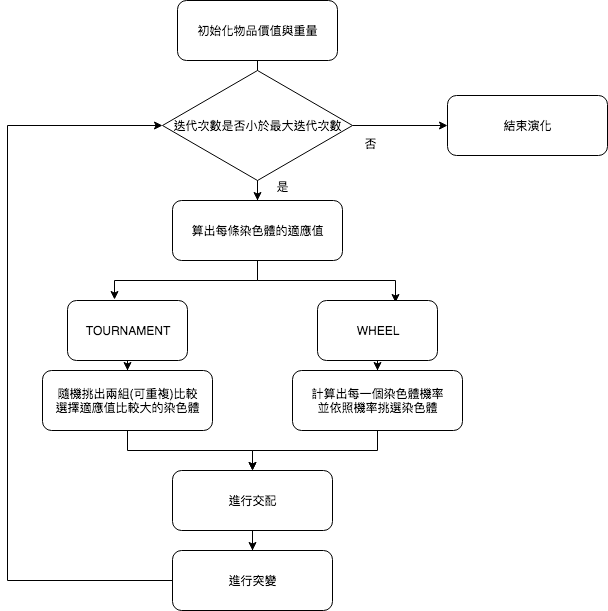
\includegraphics[width=1.0\textwidth]{image/flow2.png}
\end{figure}

\newpage
\section{趨勢圖}
{
此實驗是用演化次數500,並且個執行100次後取平均值。
\newline
可以看出WHEEL略微領先TOURNAMENT,提早到達最佳解。
\begin{figure}[ht]
\centering
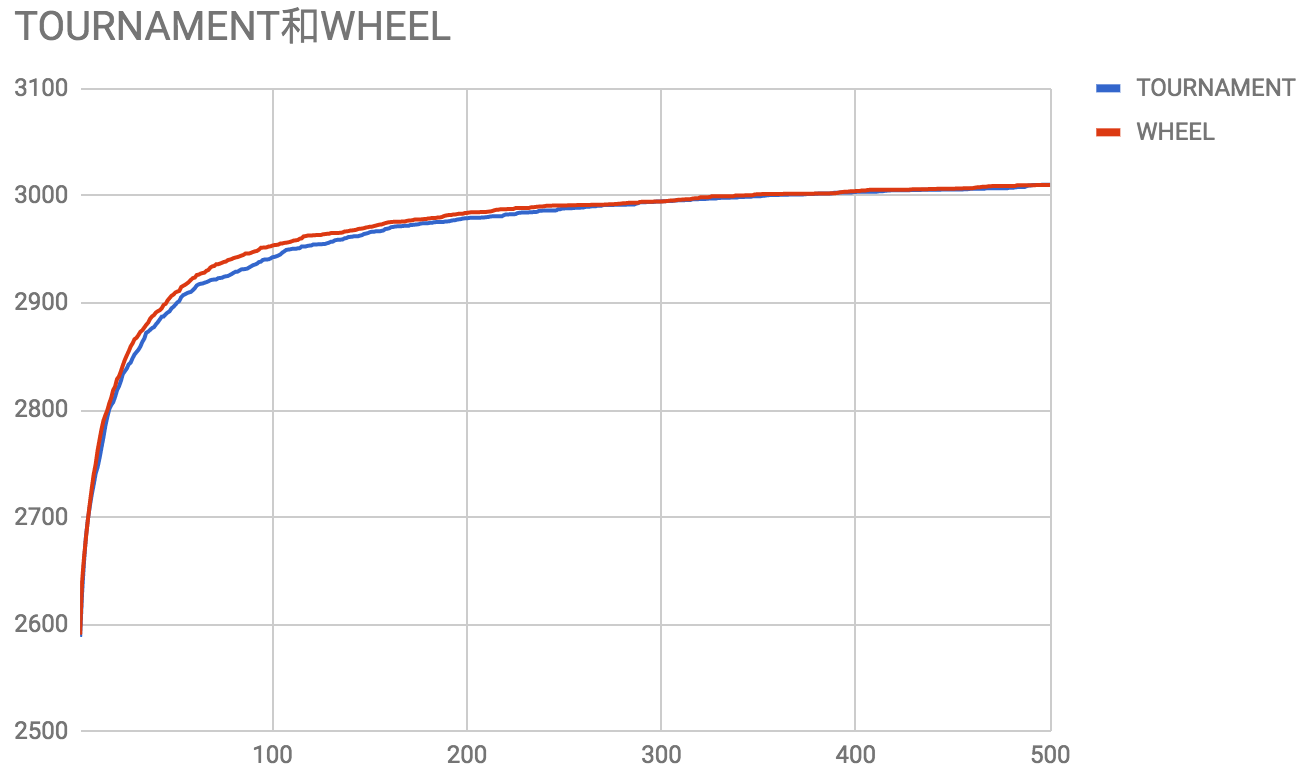
\includegraphics[width=1.0\textwidth]{image/trend.png}
\end{figure}

\section{結論}
{
1. 雖然在趨勢圖上WHEEL比TOURNMENT比較快到最佳解,但因為間距只有一些,所以可能背包問題比較難區分哪個選擇方式是比較好的。
\newline
2. 	執行速度上,TOURNMENT就真的比WHEEL快些,如果再更複雜的問題上,差距可能會更加明顯。
\newline
a. TOURNAMENT spend time = 1133ms
\newline
b. WHEEL spend time = 1320ms
}

\end{document}